% =============================================================================
% Manuscrito: Navegación espacial en personas con discapacidad visual
% Revista: Universitas Psychologica — Pontificia Universidad Javeriana
% Formato: APA 7a edición
% =============================================================================
\documentclass[12pt,letterpaper]{article}

% --- Fuente Times New Roman ---
\usepackage{mathptmx}
\usepackage[T1]{fontenc}
\usepackage[utf8]{inputenc}

% --- Idioma ---
\usepackage[english,spanish,es-tabla]{babel}
\usepackage{csquotes}

% --- Márgenes 2.5 cm ---
\usepackage[margin=2.5cm]{geometry}

% --- Interlineado doble ---
\usepackage{setspace}
\doublespacing

% --- Bibliografía APA 7 ---
\usepackage[style=apa,backend=biber,sortcites=true,sorting=nyt,language=spanish]{biblatex}
\DeclareLanguageMapping{spanish}{spanish-apa}
\addbibresource{referencias.bib}

% --- Figuras y tablas ---
\usepackage{graphicx}
\graphicspath{{figuras/}}
\usepackage{booktabs}
\usepackage{float}
\usepackage[font=small,labelfont=bf]{caption}

% --- Otros ---
\usepackage{amsmath}
\usepackage{hyperref}
\hypersetup{
    colorlinks=true,
    linkcolor=black,
    citecolor=black,
    urlcolor=blue,
    hidelinks
}
\usepackage{microtype}

% --- Formato de secciones sin numeración (estilo APA) ---
\setcounter{secnumdepth}{0}

% =============================================================================
\begin{document}

% --- TÍTULO ---
\begin{center}
{\Large\bfseries Cognición corporeizada y navegación espacial sin visión: El rol de las acciones motoras en la integración de trayectoria en personas con discapacidad visual}

\vspace{1cm}

{\large Mateo Belalcázar$^{1}$ y Yenny Otálora$^{1}$}

\vspace{0.5cm}

$^{1}$Facultad de Psicología, Universidad del Valle, Cali, Colombia

\vspace{0.5cm}

Correspondencia: mateo.belalcazar@correounivalle.edu.co

\end{center}

\vspace{1cm}

% --- RESUMEN EN ESPAÑOL ---
\section{Resumen}

Desde la perspectiva de la cognición corporeizada, las acciones motoras no son meros outputs de representaciones espaciales precomputadas, sino que participan activamente en su construcción. Este estudio evaluó el efecto de distintas claves sensoriales y motoras sobre la integración de trayectoria en personas con discapacidad visual adquirida (DV, $n = 15$) y videntes con ojos vendados (NDV, $n = 13$) mediante un paradigma de completación de triángulos. Se manipularon cuatro modalidades sensoriales: cinestésica-vestibular (línea base), tacto pasivo, interacción funcional con objetos y control (acciones en el aire sin objetos). Los resultados mostraron una interacción significativa entre la condición de experticia y la modalidad sensorial ($F(3,78) = 4.317$, $p = .007$, $\eta^2_p = .142$). El grupo DV navegó con precisión constante independientemente de la modalidad, mientras que el grupo NDV mejoró significativamente en la condición de control, igualando al grupo DV ($d = 0.03$). Análisis complementarios revelaron que este efecto opera sobre el sesgo direccional, no sobre la precisión total. Estos hallazgos apoyan la tesis de que las acciones motoras estructuran la representación espacial durante la navegación, y que la experiencia sin visión promueve la internalización de estrategias de navegación corporeizada.

\textbf{Palabras clave:} cognición corporeizada, navegación espacial, discapacidad visual, integración de trayectoria, integración multisensorial, completación de triángulos

\newpage

% --- ABSTRACT IN ENGLISH ---
\begin{otherlanguage}{english}
\section{Abstract}

From the perspective of embodied cognition, motor actions are not mere outputs of precomputed spatial representations but actively participate in their construction. This study examined the effect of different sensory and motor cues on path integration in people with acquired visual impairment (VI, $n = 15$) and blindfolded sighted controls (SC, $n = 13$) using a triangle completion paradigm. Four sensory modalities were manipulated: kinesthetic-vestibular (baseline), passive touch, functional interaction with objects, and control (actions in the air without objects). Results showed a significant interaction between expertise condition and sensory modality ($F(3,78) = 4.317$, $p = .007$, $\eta^2_p = .142$). The VI group navigated with constant accuracy regardless of modality, whereas the SC group improved significantly in the control condition, matching the VI group ($d = 0.03$). Complementary analyses revealed that this effect operates on directional bias rather than overall precision. These findings support the thesis that motor actions structure spatial representation during navigation, and that experience without vision promotes the internalization of embodied navigation strategies.

\textbf{Keywords:} embodied cognition, spatial navigation, visual impairment, path integration, multisensory integration, triangle completion
\end{otherlanguage}

\newpage

% =============================================================================
% INTRODUCCIÓN
% =============================================================================
\section{Introducción}

% P1: Navegación espacial sin visión (300 pal.)
La navegación espacial ---la capacidad de desplazarse de un punto a otro en el entorno--- constituye una función cognitiva fundamental para la autonomía y supervivencia humana. Cuando la visión no está disponible, el sistema nervioso debe apoyarse en fuentes de información alternativas para mantener una representación actualizada de la posición y orientación del cuerpo en el espacio. El mecanismo principal que sustenta esta capacidad es la integración de trayectoria (\textit{path integration}), un proceso computacional mediante el cual el organismo estima continuamente su posición a partir de señales generadas por el propio movimiento \parencite{OKeefe1978,Loomis2012}. Este proceso depende fundamentalmente de señales vestibulares, propioceptivas y de copia eferente motora que se originan durante la locomoción \parencite{Cullen2019}. Las señales vestibulares informan sobre aceleraciones lineales y angulares de la cabeza; las propioceptivas, sobre la configuración y movimiento de las articulaciones; y la copia eferente proporciona una predicción de las consecuencias sensoriales del comando motor emitido. La integración de estas señales permite al navegante construir una estimación interna de la distancia recorrida, los giros realizados y la dirección relativa al punto de origen. Sin embargo, la integración de trayectoria es inherentemente ruidosa: los errores se acumulan con la distancia, y la precisión del sistema depende críticamente de la calidad y diversidad de las fuentes sensoriales disponibles \parencite{Loomis2012,Zhou2022}. Esto plantea el problema de cómo un navegante sin visión puede mejorar la precisión de su sistema de integración de trayectoria, y qué papel desempeñan las acciones corporales en este proceso.

% P2: Cognición corporeizada e integración multisensorial (350 pal.)
La cognición corporeizada (\textit{embodied cognition}) ofrece un marco teórico para abordar esta pregunta. Desde esta perspectiva, la cognición no es un proceso abstracto confinado al cerebro, sino que está moldeada ---y en parte constituida--- por la morfología del cuerpo, sus sistemas sensoriales y sus capacidades motoras \parencite{Shapiro2019,Wilson2002}. Aplicado a la navegación espacial, el enfoque corporeizado propone que las acciones motoras no simplemente ejecutan planes espaciales precomputados, sino que \textit{estructuran} las representaciones del espacio que se van formando durante el desplazamiento \parencite{HerasEscribano2021}. En otras palabras, el cuerpo en movimiento no es un vehículo pasivo que transporta al sistema cognitivo a través del espacio, sino un recurso computacional activo que contribuye a la construcción de la representación espacial misma.

Esta perspectiva converge con la investigación sobre integración multisensorial en navegación. El cerebro pondera dinámicamente múltiples fuentes sensoriales según su fiabilidad relativa, siguiendo principios compatibles con la inferencia bayesiana óptima \parencite{Loomis2012,Zhou2022}. Cuando una fuente sensorial se pierde o degrada (como la visión), el sistema recalibra los pesos asignados a las fuentes restantes. Crucialmente, la evidencia empírica demuestra que el movimiento activo produce representaciones espaciales cualitativamente diferentes a las generadas por el transporte pasivo \parencite{Chance1998,Waller2004}. La locomoción activa integra señales propioceptivas, vestibulares y de copia eferente en un paquete sensoriomotor coherente que no está disponible durante el desplazamiento pasivo. Además, la integración multisensorial durante la marcha mejora la estimación de distancias recorridas \parencite{Campos2012}. Estos hallazgos sugieren un punto de convergencia entre la cognición corporeizada y la integración multisensorial: la acción motora no solo genera información propioceptiva adicional, sino que \textit{organiza} la integración de múltiples canales sensoriales durante la navegación, proporcionando un marco temporal y espacial que vincula las distintas señales en una representación unificada.

% P3: Discapacidad visual como experimento natural (300 pal.)
La discapacidad visual constituye un experimento natural para estudiar la navegación corporeizada. Las personas con discapacidad visual deben navegar cotidianamente sin acceso a la información visual que los videntes utilizan para calibrar y corregir su sistema de integración de trayectoria. Esta experiencia prolongada genera profundas adaptaciones en el sistema de navegación. A nivel conductual, las personas con discapacidad visual desarrollan estrategias compensatorias que les permiten alcanzar niveles de desempeño espacial comparables a los de personas videntes, un patrón descrito por el modelo convergente de la cognición espacial sin visión \parencite{Giudice2018}. A nivel neural, la plasticidad cross-modal reorganiza la corteza occipital para procesar información espacial proveniente de modalidades no visuales, incluyendo tacto, audición y propiocepción \parencite{Bleau2022meta,Chebat2020,Mowad2020}. Esta reorganización activa redes de navegación similares a las observadas en personas videntes ---corteza parietal posterior, campos oculares frontales, complejo hipocampal--- complementadas por el reclutamiento de áreas occipitales \parencite{Bleau2022meta}.

Desde una perspectiva corporeizada, las personas con discapacidad visual representan un caso paradigmático de navegación corporeizada internalizada. Al no poder depender de la visión para la actualización espacial, han desarrollado una dependencia eficiente de las señales generadas por su propio cuerpo ---vestibulares, propioceptivas, hápticas--- para construir y mantener representaciones espaciales funcionales. Estudios recientes confirman que este procesamiento eficiente de claves egocéntricas corporales sustenta el rendimiento superior observado en condiciones de navegación guiada \parencite{Shafique2024}, y que la competencia espacial sin visión puede igualar o incluso superar a la de personas videntes en tareas que dependen de información táctil \parencite{Szubielska2024}.

% P4: Claves táctiles y de acción en navegación (250 pal.)
La información proporcionada por el contacto con objetos del entorno durante la navegación constituye una fuente sensorial particularmente relevante. Las claves hápticas y táctiles pueden apoyar la construcción de representaciones espaciales funcionales tanto en personas con discapacidad visual como en videntes \parencite{Tivadar2023,Ottink2022map,Bleau2023}. Sin embargo, no toda la información táctil contribuye de la misma manera. La distinción entre tacto pasivo (tocar un objeto sin un propósito funcional) e interacción activa (usar un objeto funcionalmente) es teóricamente significativa. La exploración activa con dispositivos táctiles activa circuitos hipocampales y parahipocampales de manera proporcional al grado de participación motora, no a la mera recepción de información sensorial \parencite{Chebat2020}. Además, la información táctil tridimensional proporcionada por la interacción con objetos reales genera representaciones más ricas que las superficies planas \parencite{Bleau2023}. Estos hallazgos plantean una pregunta que permite disociar las predicciones de la cognición corporeizada y la integración multisensorial: ¿las acciones motoras por sí solas (sin contacto con objetos) son suficientes para mejorar la representación espacial durante la navegación, o se requiere el contacto multimodal con objetos del entorno? La cognición corporeizada predice que la acción motora basta para reestructurar la representación; la integración multisensorial sugiere que a mayor riqueza sensorial, mejor representación.

% P5: El presente estudio (200 pal.)
El presente estudio abordó esta pregunta mediante un diseño factorial mixto 2$\times$4 que manipuló cuatro condiciones sensoriales-motoras durante una tarea de completación de triángulos, comparando personas con discapacidad visual adquirida (DV) con videntes con ojos vendados (NDV). Las condiciones disociaron sistemáticamente la acción motora del contacto con objetos: (a) cinestésica-vestibular (línea base, sin objetos ni acciones adicionales), (b) tacto pasivo (tocar objetos sin usarlos), (c) interacción funcional (usar objetos), y (d) control (realizar acciones en el aire, sin objetos). Desde la cognición corporeizada, se hipotetizó que las condiciones que involucran acciones motoras ---interacción funcional y control--- mejorarían el desempeño del grupo NDV, incluso sin contacto con objetos, porque la acción motora reestructura la representación espacial. Desde la integración multisensorial, se predijo que las condiciones con mayor riqueza sensorial ---tacto pasivo e interacción funcional--- producirían mejores representaciones por la adición de canales informativos. Finalmente, se hipotetizó que el grupo DV mostraría menor dependencia de la modalidad sensorial, reflejando la internalización de estrategias de navegación corporeizada que no requieren fuentes externas de información.

% =============================================================================
% MÉTODO
% =============================================================================
\section{Método}

\subsection{Participantes}

Participaron 28 adultos distribuidos en dos grupos: 15 personas con discapacidad visual adquirida (DV; 11 hombres, 4 mujeres; $M_{\text{edad}} = 43.53$ años, $DE = 13.16$) y 13 personas sin discapacidad visual (NDV; 9 hombres, 4 mujeres; $M_{\text{edad}} = 37.69$ años, $DE = 14.78$). Los participantes del grupo DV fueron reclutados a través del servicio de oftalmología del Hospital Universitario del Valle (HUV, Cali, Colombia) y presentaban ceguera total o percepción de luz sin funcionalidad visual, con un promedio de $8.67$ años sin visión ($DE = 6.44$). El grupo NDV fue reclutado por conveniencia, pareado por edad, sexo y escolaridad. Los grupos no difirieron significativamente en edad ($t = 1.097$, $p = .283$, $d = 0.42$), escolaridad ($t = -0.628$, $p = .536$, $d = -0.23$) ni distribución por sexo ($\chi^2(1) = 0.000$, $p = 1.000$). Todos los participantes proporcionaron consentimiento informado. El estudio fue aprobado por el comité de ética de la Universidad del Valle.

\subsection{Diseño}

Se empleó un diseño cuasi-experimental factorial mixto. El factor entre-sujetos fue la condición de experticia (CE: DV vs. NDV). Los factores intra-sujetos fueron la organización por forma (OF: triángulos agudos con ángulo $< 45^{\circ}$ vs. obtusos con ángulo $> 90^{\circ}$), la organización por tamaño (OT: distancia de retorno de 2 m vs. 4 m) y la modalidad sensorial (MS: cinestésica-vestibular, tacto pasivo, interacción funcional, control). Cada participante completó $2 \times 2 \times 4 = 16$ ensayos. Las variables dependientes fueron el error de posición con signo (distancia en centímetros entre el punto de origen y el punto alcanzado por el participante, con valores positivos indicando sobreestimación y negativos subestimación) y el error de estimación angular (diferencia en grados entre la dirección estimada y la dirección ideal de retorno).

\subsection{Materiales e instrumento}

Se utilizó el paradigma de completación de triángulos \parencite{McLaren2022}. Los participantes caminaban dos segmentos de un triángulo (guiados por el experimentador) y debían estimar y completar el tercer segmento para regresar al punto de origen. Los triángulos variaron en su geometría: triángulos agudos (ángulo de giro $< 45^{\circ}$) y obtusos (ángulo de giro $> 90^{\circ}$), con distancias de retorno de 2 m y 4 m. Las trayectorias se ejecutaron en un espacio amplio y plano, libre de obstáculos y de claves auditivas direccionales.

En cada ensayo, se colocaron objetos cotidianos (p. ej., una taza, una botella, un timbre) en los vértices del triángulo. Las cuatro modalidades sensoriales definieron la forma de interacción con estos objetos:

\begin{enumerate}
    \item \textbf{Cinestésica-vestibular (línea base):} el participante caminaba los dos segmentos sin tocar ni interactuar con ningún objeto. Solo disponía de información vestibular, propioceptiva y de copia eferente motora generada por la locomoción.
    \item \textbf{Tacto pasivo:} al llegar a cada vértice, el participante tocaba el objeto presente sin realizar ninguna acción funcional con él. Se añadía información háptica sobre la forma, textura y ubicación del objeto.
    \item \textbf{Interacción funcional:} al llegar a cada vértice, el participante usaba funcionalmente el objeto (p. ej., beber de la taza, hacer sonar el timbre). Se combinaba información háptica con programas motores específicos de acción sobre objetos.
    \item \textbf{Control:} al llegar a cada vértice, el participante realizaba una acción motora en el aire (p. ej., simular beber, simular hacer sonar un timbre) sin tocar ningún objeto. Se ejecutaban programas motores sin retroalimentación háptica del objeto.
\end{enumerate}

\subsection{Procedimiento}

Los participantes del grupo NDV fueron vendados antes de iniciar la sesión experimental y permanecieron sin visión durante toda la tarea. Cada sesión comenzó con una fase de familiarización en la que el participante completó dos ensayos de práctica (no incluidos en el análisis) para comprender la tarea. El experimentador guiaba al participante por los dos primeros segmentos del triángulo, indicando verbalmente cada giro. Al finalizar el segundo segmento, se le pedía que se detuviera, señalara con el brazo extendido la dirección estimada al punto de origen (registro del error angular) y caminara en línea recta hacia dicho punto (registro del error de posición). La posición final fue registrada con cinta métrica.

El orden de presentación de las cuatro modalidades sensoriales fue contrabalanceado entre participantes utilizando un cuadrado latino. Dentro de cada modalidad, los cuatro triángulos (2 formas $\times$ 2 tamaños) se presentaron en orden aleatorio. En las condiciones de tacto pasivo, interacción funcional y control, el experimentador entregaba instrucciones específicas antes de cada bloque. La sesión completa duró aproximadamente 45 minutos por participante.

\subsection{Plan de análisis}

Todos los análisis estadísticos se realizaron en Python 3.11 utilizando las bibliotecas \textit{pingouin} \parencite{Vallat2018}, \textit{scipy} y \textit{statsmodels}. El análisis principal fue un ANOVA de medidas repetidas con un factor entre-sujetos (CE) y un factor intra-sujetos (MS), colapsando sobre forma y tamaño. Este modelo se justificó dado que el interés teórico central recaía en la interacción CE $\times$ MS. Se reportó previamente un ANOVA factorial completo 2$\times$2$\times$2$\times$4 para verificar que las interacciones de orden superior no invalidaran el colapso.

Las comparaciones post hoc se realizaron con corrección de Bonferroni. Los efectos simples de modalidad se analizaron separadamente dentro de cada grupo, y las comparaciones entre grupos se realizaron dentro de cada modalidad. Los tamaños del efecto se reportaron como $\eta^2_p$ para ANOVAs y $d$ de Cohen para comparaciones entre grupos.

Como análisis complementarios, se examinaron: (a) el sesgo direccional mediante pruebas $t$ de una muestra contra cero, (b) el error absoluto para distinguir efectos sobre calibración vs. precisión total, (c) la variabilidad intra-participante como variable dependiente, y (d) el error de estimación angular. La robustez de los resultados se evaluó mediante ANOVA de rangos alineados \parencite[ART;][]{Wobbrock2011,Elkin2021}. Adicionalmente, se calcularon factores de Bayes ($BF_{10}$) como complemento a la inferencia frecuentista \parencite{vanDoorn2021}.

% =============================================================================
% RESULTADOS
% =============================================================================
\section{Resultados}

\subsection{ANOVA factorial completo}

El ANOVA factorial mixto 2(CE) $\times$ 2(OF) $\times$ 2(OT) $\times$ 4(MS) sobre el error de posición con signo reveló un efecto principal significativo de la condición de experticia, $F(1, 26) = 4.695$, $p = .040$, $\eta^2_p = .153$, indicando que el grupo DV cometió errores menores que el grupo NDV. La interacción CE $\times$ factor intra-sujetos combinado fue significativa, $F(15, 390) = 3.964$, $p < .001$, $\eta^2_p = .132$ (con corrección de Greenhouse-Geisser, $\varepsilon = 0.485$).

La descomposición por factores reveló interacciones significativas CE $\times$ OF ($F(1, 26) = 6.377$, $p = .018$, $\eta^2_p = .197$), CE $\times$ OT ($F(1, 26) = 8.738$, $p = .007$, $\eta^2_p = .252$) y, crucialmente, CE $\times$ MS ($F(3, 78) = 4.317$, $p = .007$, $\eta^2_p = .142$). Las interacciones de orden superior CE $\times$ OF $\times$ OT ($F(3, 78) = 5.755$, $p = .001$), CE $\times$ OF $\times$ MS ($F(7, 182) = 3.431$, $p = .002$) y CE $\times$ OT $\times$ MS ($F(7, 182) = 5.839$, $p < .001$) también fueron significativas. Dado que el interés teórico central recaía en cómo las distintas modalidades sensoriales afectan diferencialmente a cada grupo, y que las interacciones con forma y tamaño reflejaban patrones geométricos secundarios, los análisis subsiguientes se focalizaron en el modelo colapsado CE $\times$ MS.

\subsection{Análisis central: interacción CE $\times$ MS}

El ANOVA 2(CE) $\times$ 4(MS) sobre el error de posición con signo (promediando sobre forma y tamaño) confirmó los tres efectos: condición de experticia, $F(1, 26) = 4.695$, $p = .040$, $\eta^2_p = .153$; modalidad sensorial, $F(3, 78) = 3.690$, $p = .015$, $\eta^2_p = .124$; e interacción CE $\times$ MS, $F(3, 78) = 4.317$, $p = .007$, $\eta^2_p = .142$. La Figura~\ref{fig:interaction} muestra el patrón de esta interacción.

\begin{figure}[H]
\centering
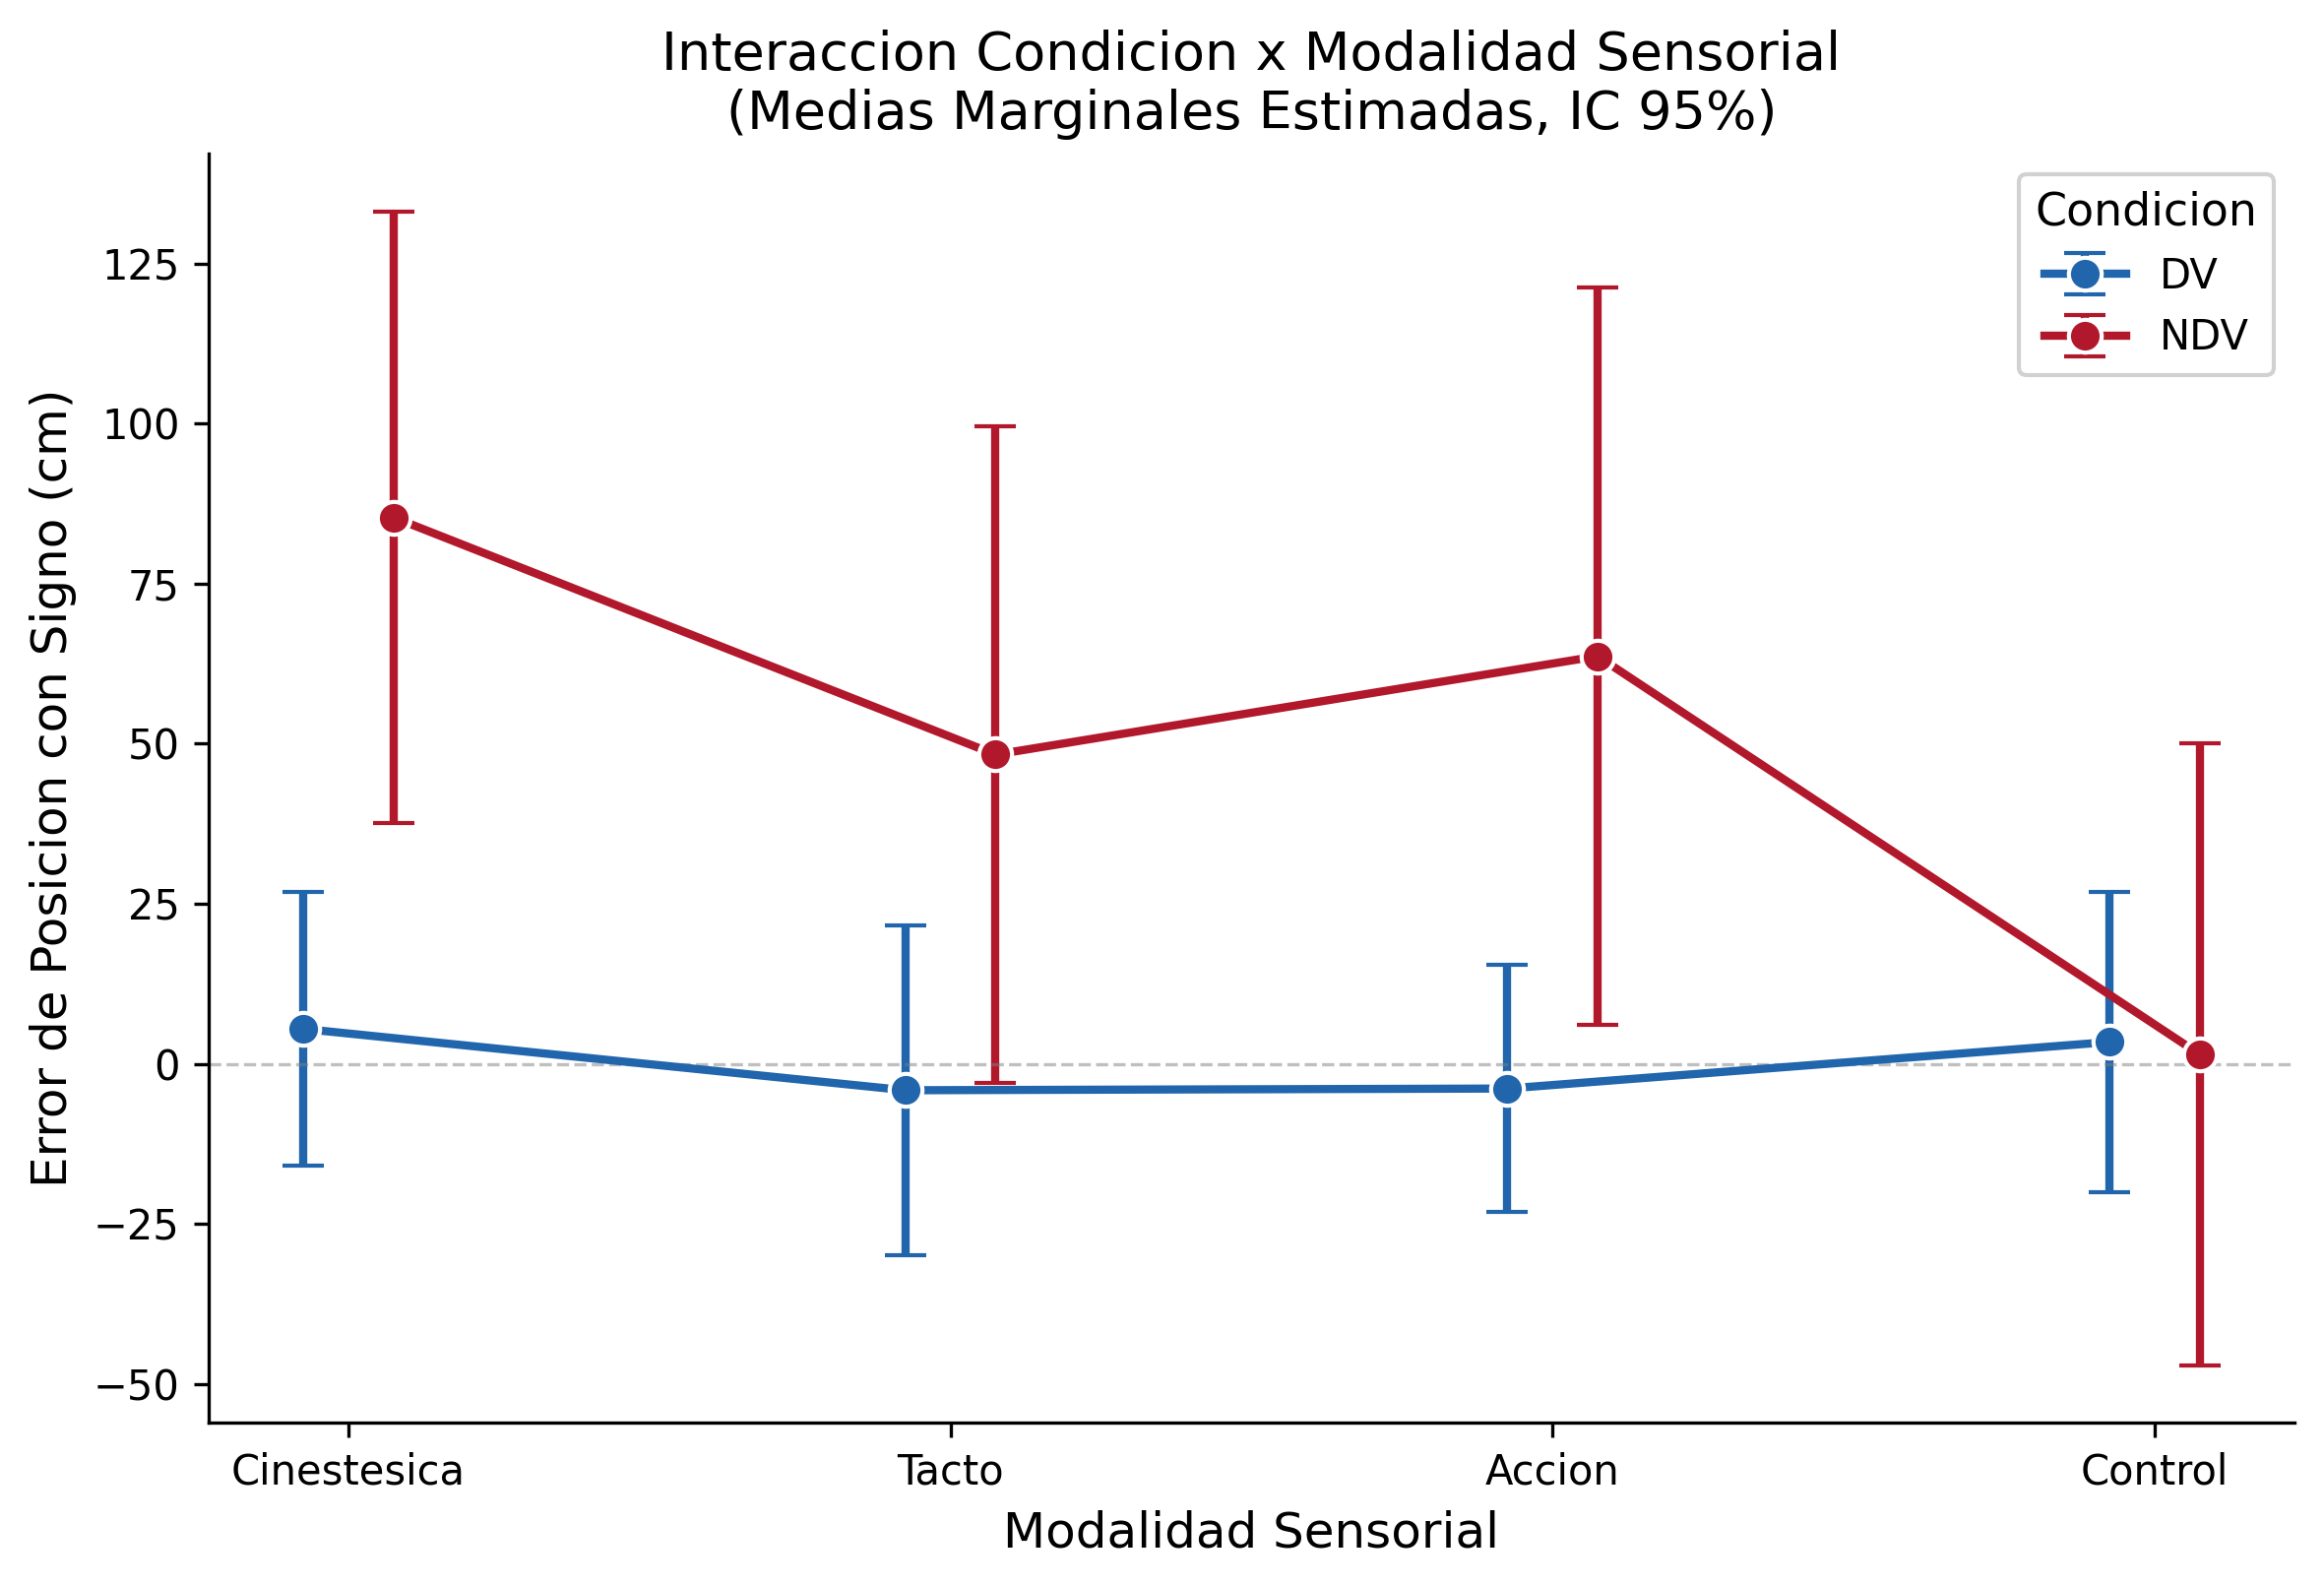
\includegraphics[width=0.85\textwidth]{fig1_interaction_CE_MS.png}
\caption{Interacción entre la condición de experticia (DV vs. NDV) y la modalidad sensorial sobre el error de posición con signo. Las barras representan medias; las líneas de error representan intervalos de confianza al 95\%. CIN = cinestésica-vestibular; TAC = tacto pasivo; ACC = interacción funcional; CTR = control (acciones en el aire). $^{**}p < .01$, $^{*}p < .05$, ns = no significativo para las comparaciones entre grupos.}
\label{fig:interaction}
\end{figure}

Las comparaciones post hoc sobre la muestra total (corrección de Bonferroni) revelaron que la única diferencia significativa entre modalidades fue cinestésica-vestibular vs. control ($t(27) = 2.871$, $p_{\text{Bonf}} = .047$, $g = 0.541$, $BF_{10} = 5.645$). Las restantes comparaciones no alcanzaron significación tras la corrección (todas $p_{\text{Bonf}} > .25$).

% --- Efectos simples ---
La descomposición de la interacción reveló patrones marcadamente diferentes en cada grupo. En el grupo DV, la modalidad sensorial no tuvo efecto sobre el error de posición, $F(3, 42) = 0.312$, $p = .816$, $\eta^2_g = .010$. Ninguna comparación post hoc fue significativa (todas $p > .42$). El grupo DV navegó con errores cercanos a cero en todas las modalidades: cinestésica ($M = 5.47$ cm, $DE = 42.24$), tacto ($M = -4.12$ cm, $DE = 50.90$), interacción funcional ($M = -3.85$ cm, $DE = 38.19$) y control ($M = 3.42$ cm, $DE = 46.33$).

En contraste, el grupo NDV mostró un efecto significativo de la modalidad, $F(3, 36) = 5.169$, $p = .004$, $\eta^2_g = .103$. Las comparaciones post hoc revelaron que la condición de control (acciones en el aire) redujo dramáticamente el error respecto a la condición cinestésica-vestibular ($t = 4.766$, $p_{\text{Bonf}} = .003$, $g = 0.917$) y respecto a la interacción funcional ($t = -3.569$, $p_{\text{Bonf}} = .023$, $g = -0.615$). El grupo NDV mostró sobreestimación sustancial en la condición cinestésica ($M = 85.35$ cm, $DE = 87.90$) y en la interacción funcional ($M = 63.67$ cm, $DE = 105.87$), mientras que en la condición de control el error medio fue prácticamente nulo ($M = 1.50$ cm, $DE = 89.29$).

Las comparaciones entre grupos dentro de cada modalidad iluminaron la interacción. En la condición cinestésica-vestibular (línea base), el grupo DV fue significativamente más preciso que el NDV ($t = -2.991$, $p = .008$, $d = -1.187$). En la condición de interacción funcional, la diferencia persistió ($t = -2.180$, $p = .046$, $d = -0.875$). En la condición de tacto pasivo, la diferencia se redujo a un nivel no significativo ($t = -1.791$, $p = .090$, $d = -0.707$). Crucialmente, en la condición de control, los grupos fueron estadísticamente indistinguibles ($t = 0.070$, $p = .945$, $d = 0.028$; Figura~\ref{fig:trajectories}).

\subsection{Estadísticas descriptivas y patrones individuales}

La Tabla~\ref{tab:descriptivos} presenta las medias y desviaciones estándar del error de posición con signo para cada grupo en las cuatro modalidades sensoriales, colapsando sobre forma y tamaño. El patrón descriptivo revela un contraste marcado entre los dos grupos. El grupo DV presentó errores medios cercanos a cero en todas las modalidades, oscilando entre $-4.12$ cm (tacto pasivo) y $5.47$ cm (cinestésica-vestibular), con desviaciones estándar relativamente homogéneas ($DE = 38$--$51$ cm). Esta distribución centrada en el origen indica que el grupo DV no presentó sesgo sistemático de sobreestimación ni de subestimación en ninguna condición, y que su sistema de integración de trayectoria operó con una calibración estable independientemente de las claves sensoriales disponibles.

\begin{table}[H]
\centering
\caption{Estadísticas descriptivas del error de posición con signo (cm) por grupo y modalidad sensorial.}
\label{tab:descriptivos}
\begin{tabular}{llrrr}
\toprule
Grupo & Modalidad & $M$ & $DE$ & $n$ \\
\midrule
DV  & Cinestésica-vestibular & 5.47   & 42.24  & 15 \\
DV  & Tacto pasivo           & $-$4.12  & 50.90  & 15 \\
DV  & Interacción funcional  & $-$3.85  & 38.19  & 15 \\
DV  & Control                & 3.42   & 46.33  & 15 \\
\addlinespace
NDV & Cinestésica-vestibular & 85.35  & 87.90  & 13 \\
NDV & Tacto pasivo           & 48.31  & 94.29  & 13 \\
NDV & Interacción funcional  & 63.67  & 105.87 & 13 \\
NDV & Control                & 1.50   & 89.29  & 13 \\
\bottomrule
\end{tabular}

\vspace{0.3cm}
\small\textit{Nota.} Valores positivos indican sobreestimación de la distancia de retorno; negativos, subestimación. DV = discapacidad visual adquirida; NDV = sin discapacidad visual.
\end{table}

El grupo NDV, en cambio, mostró un perfil diferente tanto en magnitud como en dispersión. En la condición cinestésica-vestibular (línea base), el error medio fue de $85.35$ cm ---una sobreestimación sustancial de la distancia de retorno---, acompañado de una desviación estándar elevada ($DE = 87.90$ cm). La condición de interacción funcional presentó un patrón similar ($M = 63.67$ cm, $DE = 105.87$ cm). El tacto pasivo produjo una reducción parcial del error medio ($M = 48.31$ cm), aunque con alta variabilidad ($DE = 94.29$ cm). El dato más notable es la condición de control: el error medio del grupo NDV se redujo a apenas $1.50$ cm, un valor prácticamente idéntico al del grupo DV en cualquier modalidad. Sin embargo, la desviación estándar se mantuvo elevada ($DE = 89.29$ cm), indicando que la corrección del sesgo no estuvo acompañada de una reducción equivalente en la dispersión individual.

La Figura~\ref{fig:trajectories} ilustra este patrón a nivel individual. Las trayectorias del grupo DV se distribuyen de manera simétrica alrededor del punto de origen en las cuatro modalidades, reflejando la ausencia de sesgo y la consistencia del desempeño. En el grupo NDV, las trayectorias de la condición cinestésica muestran un desplazamiento sistemático hacia la sobreestimación, con amplia dispersión. En la condición de control, las trayectorias del grupo NDV se recentran alrededor del origen ---eliminando el sesgo---, aunque mantienen una dispersión mayor que la del grupo DV. Este patrón visual confirma que las acciones motoras en el aire recalibraron el sistema de navegación del grupo NDV, corrigiendo la tendencia a sobreestimar la distancia de retorno sin necesariamente reducir la variabilidad de las respuestas individuales.

\begin{figure}[H]
\centering
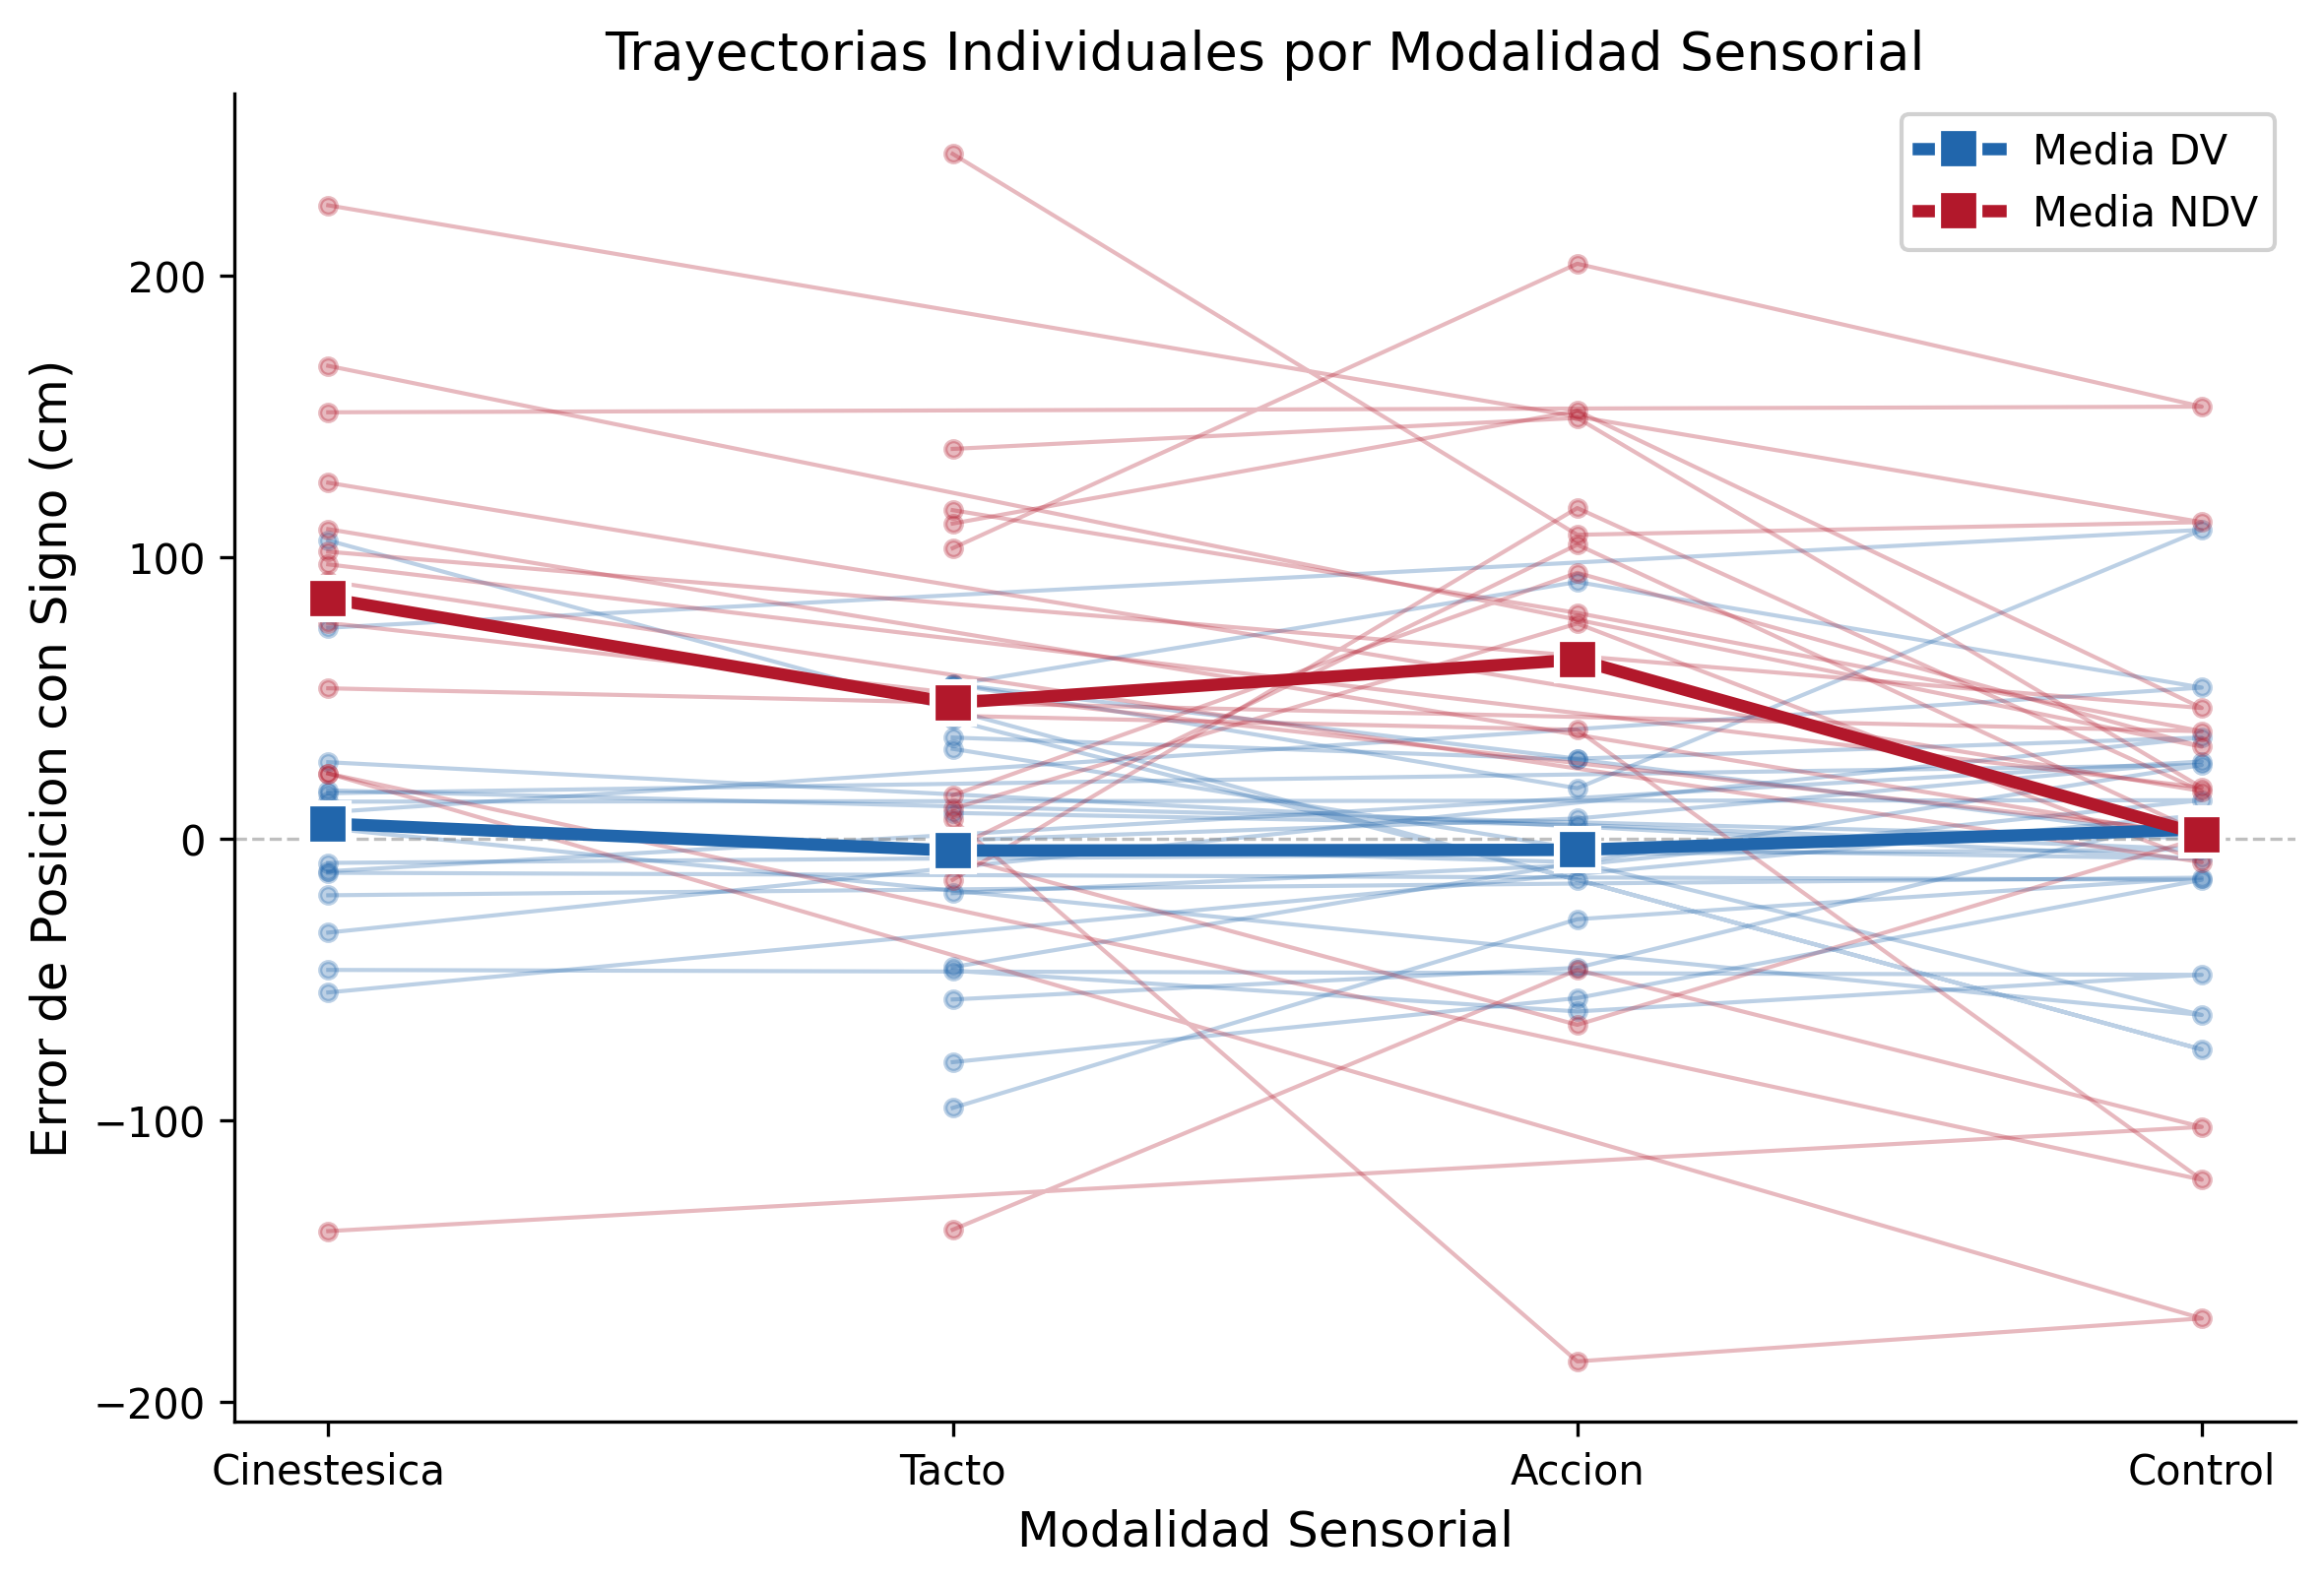
\includegraphics[width=0.85\textwidth]{fig2_individual_trajectories.png}
\caption{Trayectorias individuales de retorno por grupo y modalidad sensorial. Cada línea representa la trayectoria de un participante desde el punto final del segundo segmento hasta su estimación del punto de origen. El punto de referencia (origen real) se indica con un marcador central. El grupo DV muestra trayectorias centradas y consistentes en todas las modalidades; el grupo NDV muestra mayor dispersión y un sesgo de sobreestimación que desaparece en la condición de control.}
\label{fig:trajectories}
\end{figure}

\subsection{Sesgo direccional}

Pruebas $t$ de una muestra contra cero evaluaron si cada grupo presentaba un sesgo sistemático de sobreestimación o subestimación en cada modalidad. El grupo DV no mostró sesgo significativo en ninguna modalidad (todos $|t| < 0.501$, todos $p > .62$), indicando una calibración precisa del sistema de navegación. En contraste, el grupo NDV mostró sobreestimación significativa en la condición cinestésica-vestibular ($M = 85.35$ cm, $t(12) = 3.501$, $p = .004$, $d = 0.97$), con tendencias en la misma dirección en tacto pasivo ($M = 48.31$ cm, $p = .089$) e interacción funcional ($M = 63.67$ cm, $p = .051$). Notablemente, este sesgo desapareció completamente en la condición de control ($M = 1.50$ cm, $t(12) = 0.061$, $p = .953$, $d = 0.02$; Figura~\ref{fig:bias}). Las acciones motoras en el aire eliminaron la sobreestimación sistemática del grupo NDV.

\begin{figure}[H]
\centering
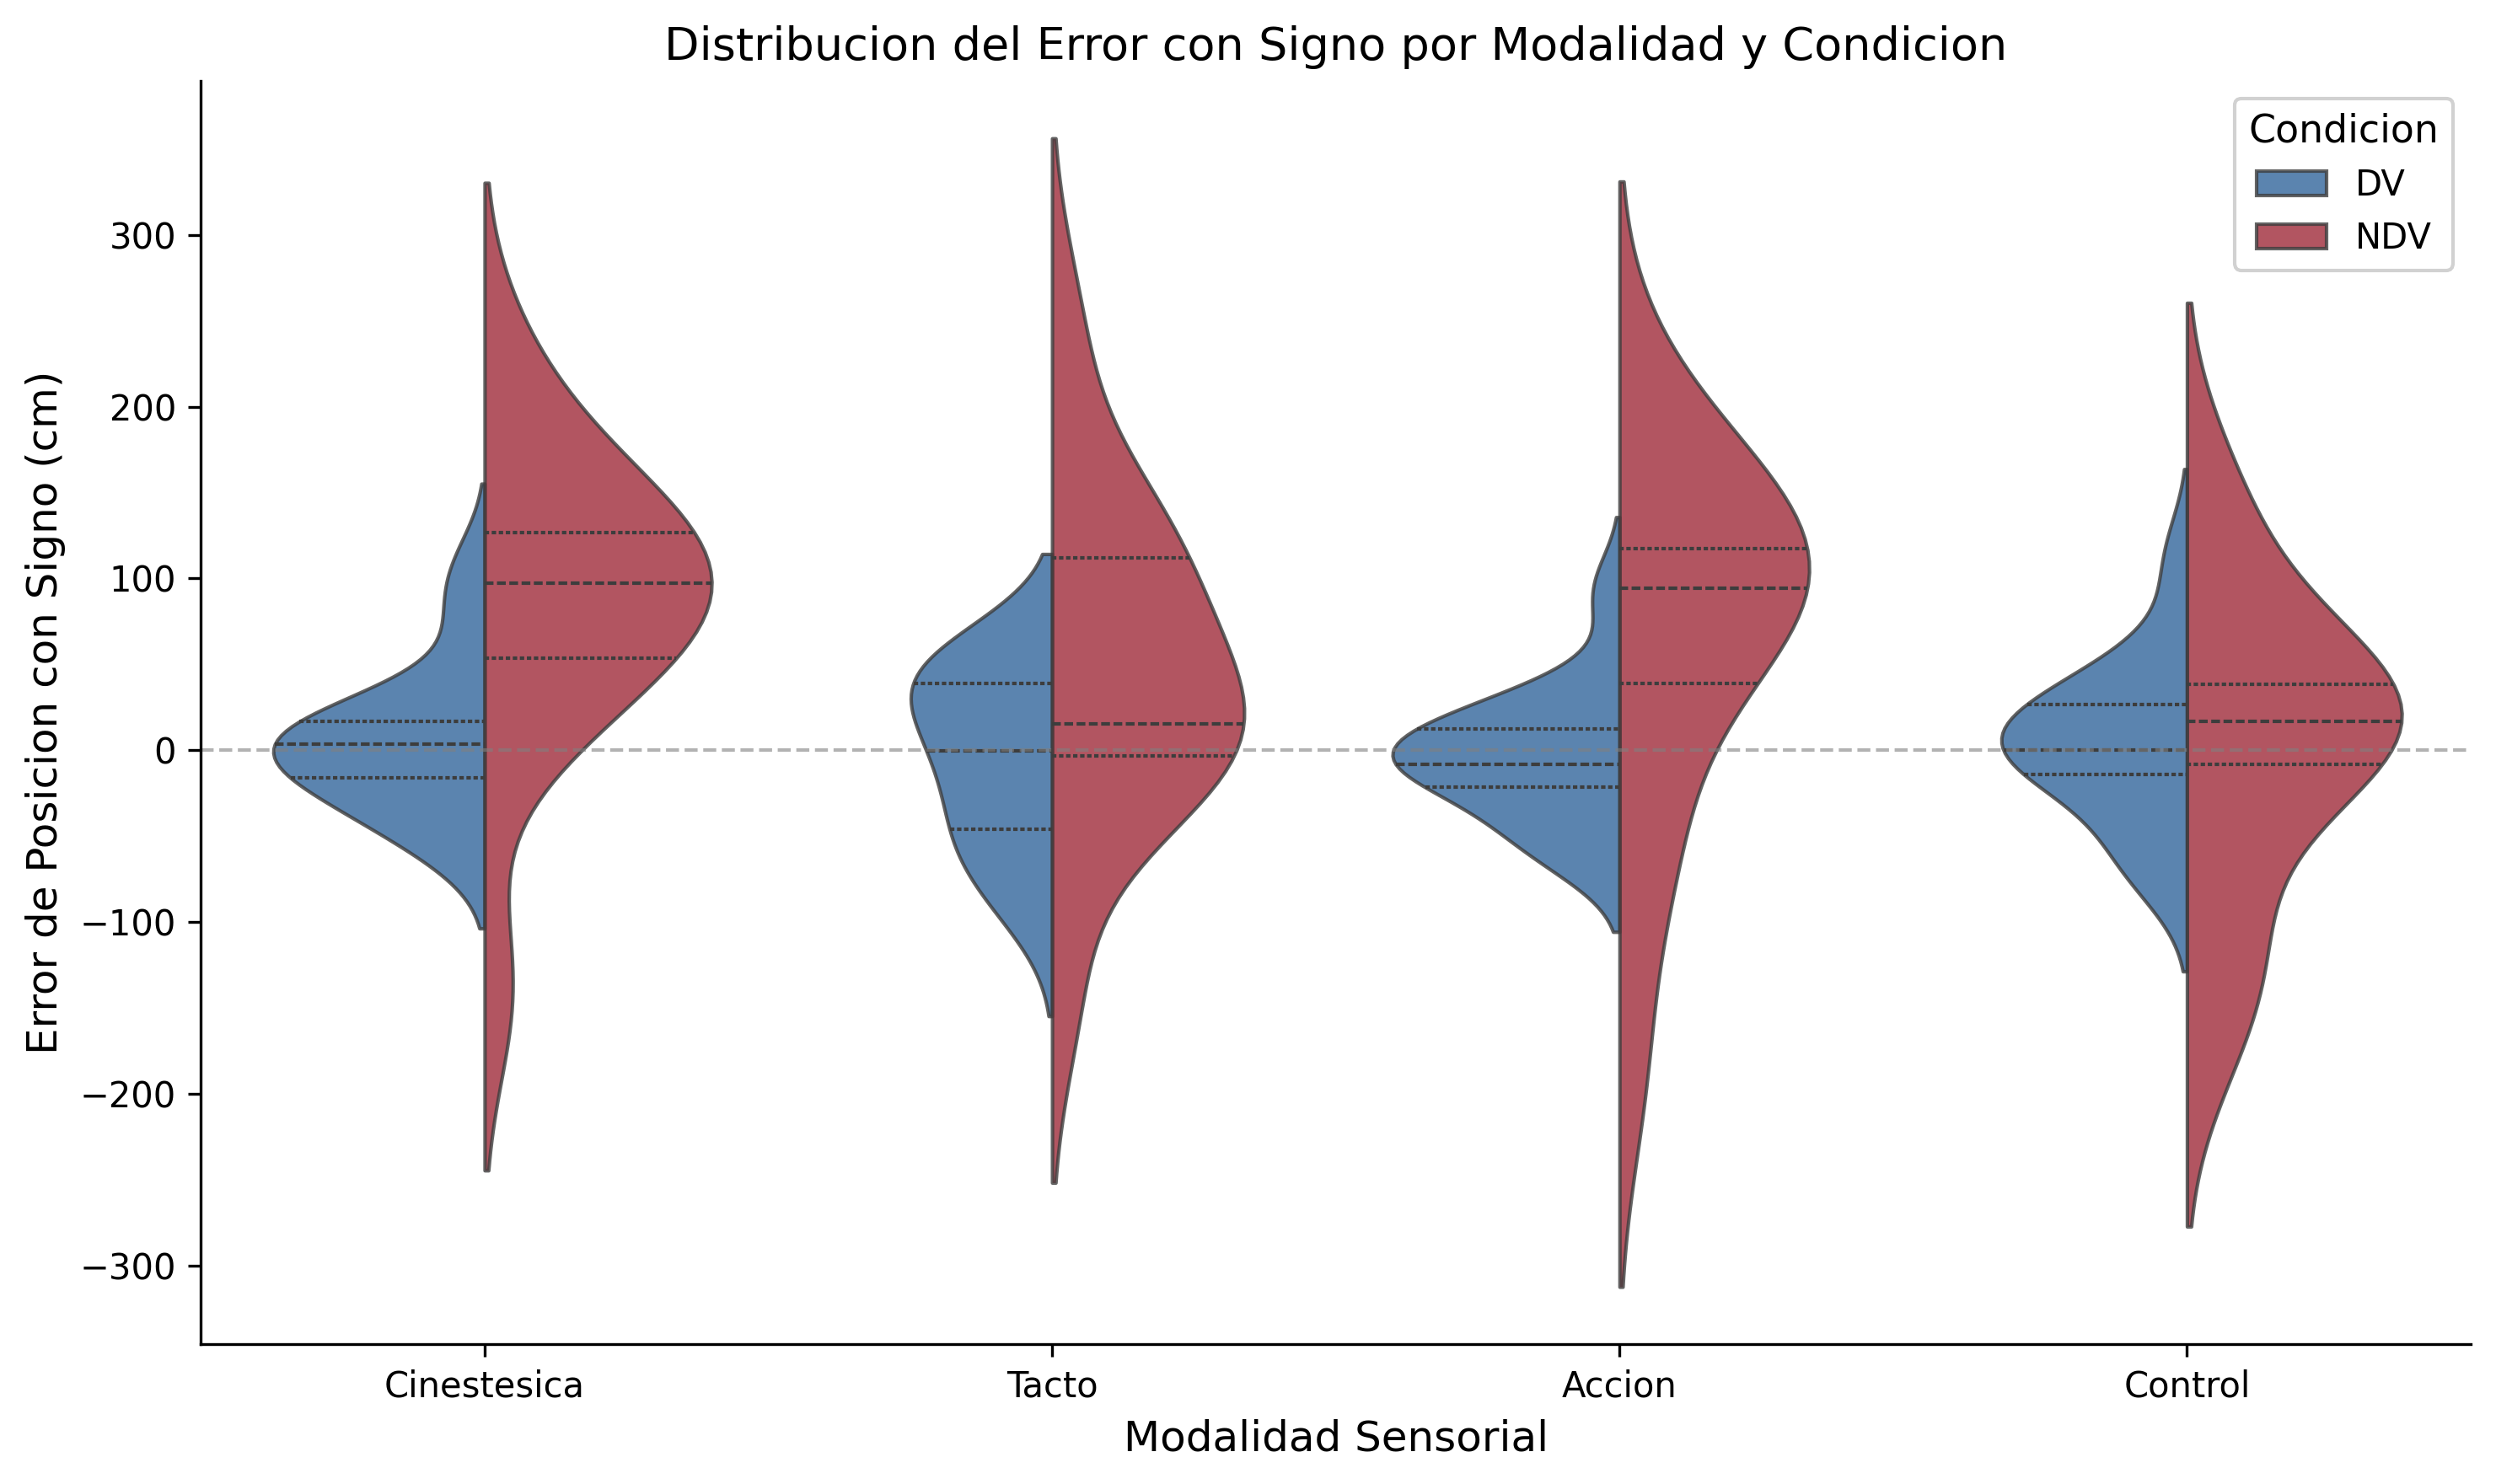
\includegraphics[width=0.85\textwidth]{fig5_error_direction.png}
\caption{Distribución del sesgo direccional (error de posición con signo) por grupo y modalidad sensorial. Los violines representan la distribución de errores; los puntos representan las medias. Valores positivos indican sobreestimación; negativos, subestimación. La línea punteada horizontal marca el cero (sin sesgo). $^{**}p < .01$ para la prueba $t$ de una muestra contra cero. El grupo NDV muestra sobreestimación significativa únicamente en la condición cinestésica-vestibular.}
\label{fig:bias}
\end{figure}

\subsection{Error absoluto vs. error con signo}

Para distinguir si la interacción CE $\times$ MS operaba sobre la calibración direccional o sobre la precisión total, se repitió el ANOVA utilizando el error absoluto ($|E|$) como variable dependiente. El efecto principal de la condición de experticia se incrementó sustancialmente, $F(1, 26) = 23.755$, $p < .001$, $\eta^2_p = .477$, y la modalidad sensorial mantuvo su efecto, $F(3, 78) = 3.657$, $p = .016$. Sin embargo, la interacción CE $\times$ MS dejó de ser significativa, $F(3, 78) = 1.182$, $p = .322$, $\eta^2_p = .044$ (Figura~\ref{fig:absolute}).

\begin{figure}[H]
\centering
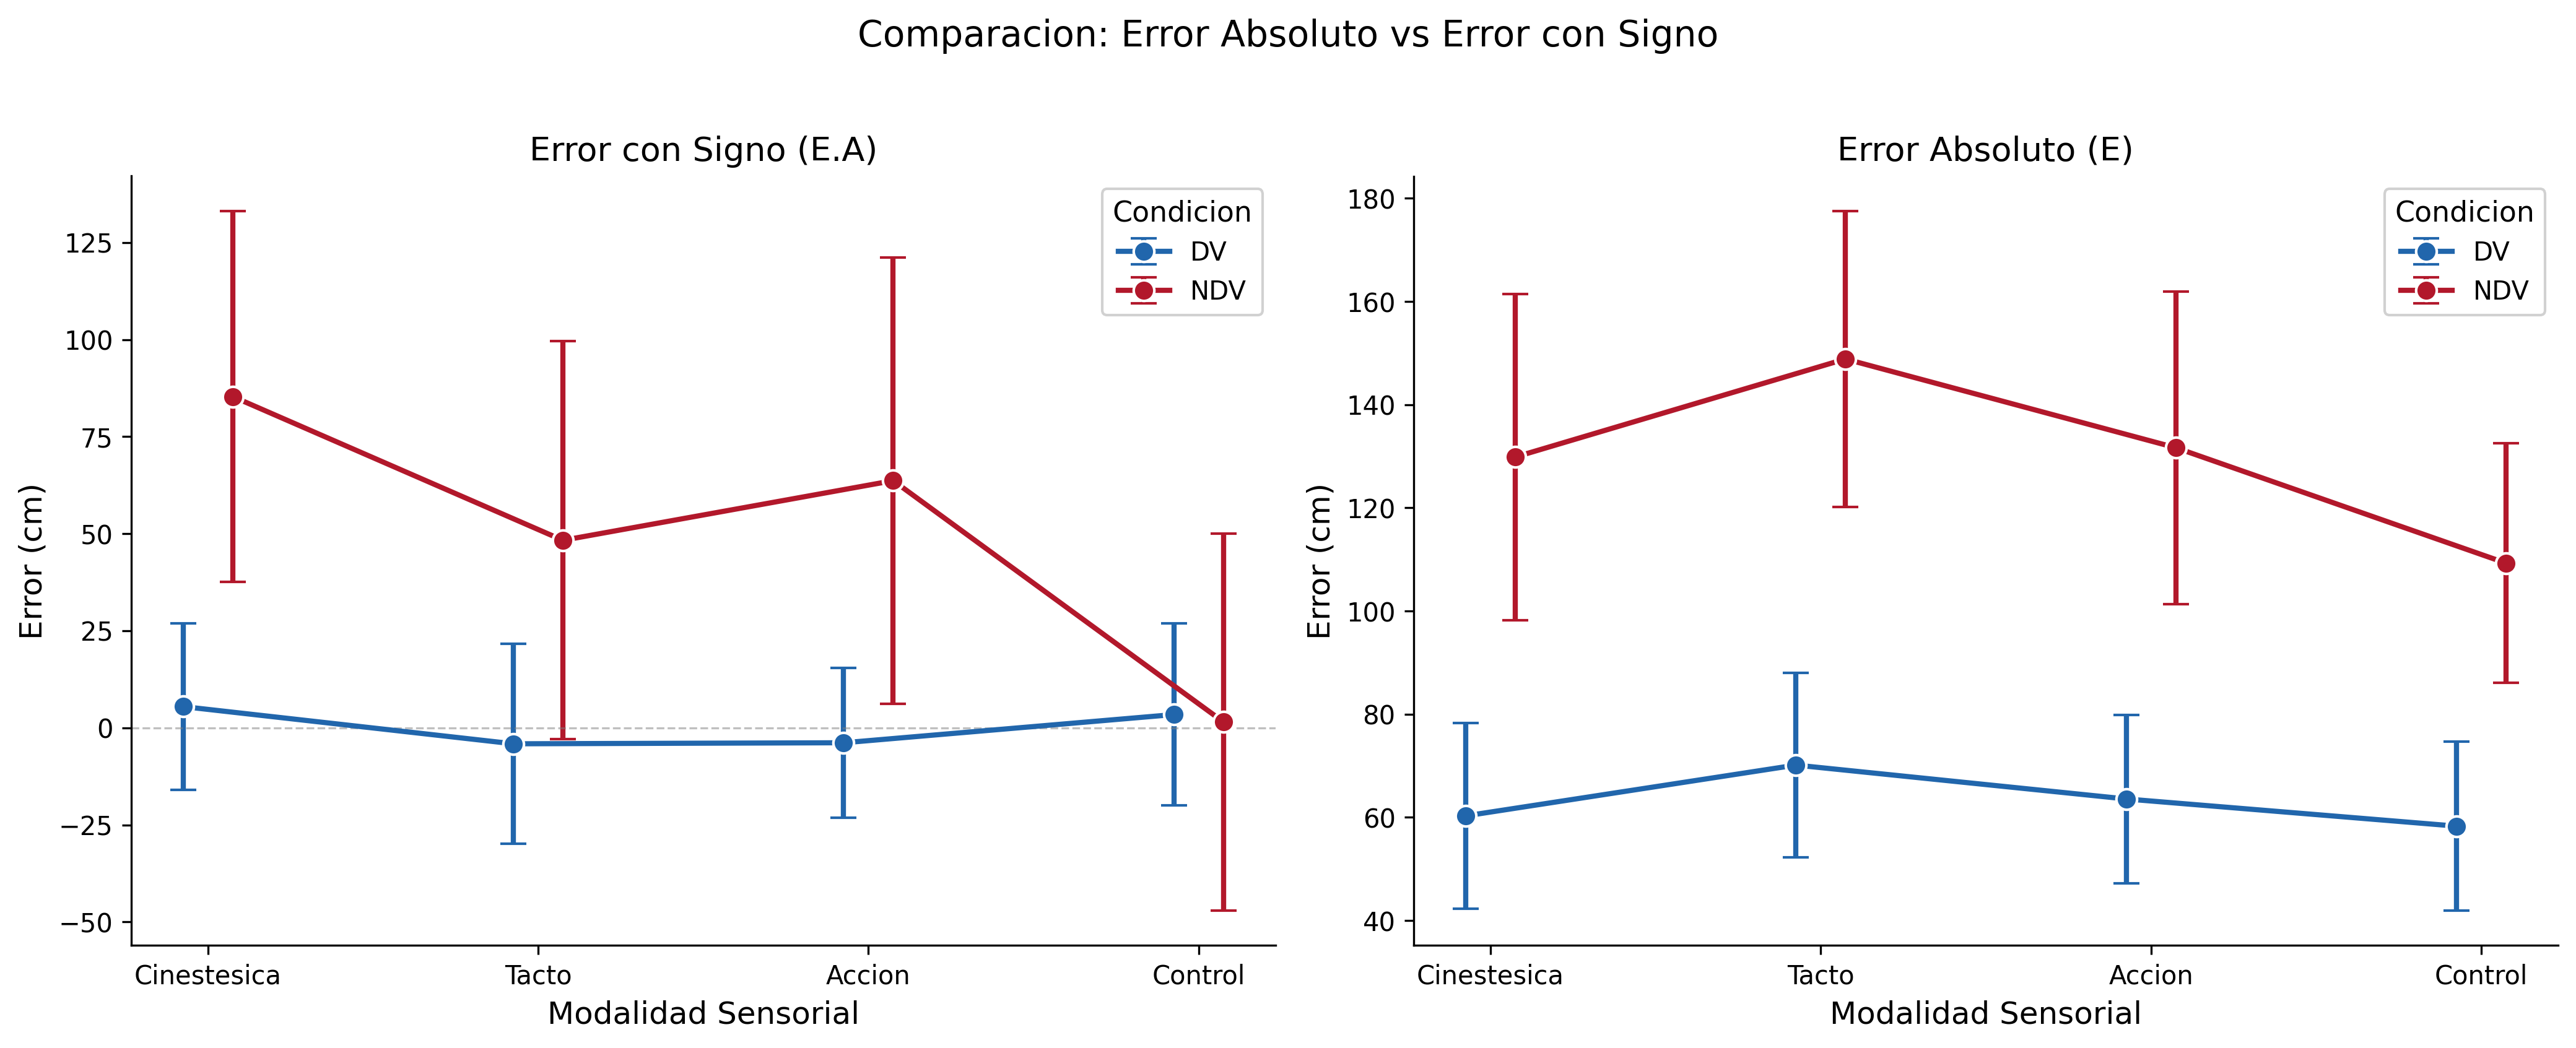
\includegraphics[width=0.85\textwidth]{fig3_absolute_vs_signed.png}
\caption{Comparación del error absoluto y el error con signo por grupo y modalidad sensorial. Panel izquierdo: error con signo (interacción CE $\times$ MS significativa, $p = .007$). Panel derecho: error absoluto (interacción no significativa, $p = .322$). Esta disociación indica que las acciones motoras corrigen el sesgo direccional del grupo NDV sin reducir la magnitud total del error.}
\label{fig:absolute}
\end{figure}

Este resultado revela que el efecto diferencial de la modalidad sensorial entre grupos se debe al sesgo direccional ---la sobreestimación sistemática del grupo NDV en la condición cinestésica---, no a diferencias en la magnitud total del error. En la condición de control, por ejemplo, el grupo NDV presentó un error absoluto medio de 109.28 cm pero un error con signo de apenas 1.50 cm, indicando que los errores positivos y negativos se cancelaron casi perfectamente. Las acciones motoras corrigieron la calibración del sistema de navegación del grupo NDV sin reducir necesariamente la dispersión de los errores individuales.

\subsection{Variabilidad}

Análisis de la consistencia intra-participante (desviación estándar de los errores de posición a través de las cuatro condiciones geométricas) revelaron que el grupo NDV fue significativamente más variable que el grupo DV en tres de cuatro modalidades: cinestésica ($t = -2.529$, $p = .018$, $d = -0.97$), tacto pasivo ($t = -4.114$, $p < .001$, $d = -1.58$) y control ($t = -3.010$, $p = .007$, $d = -1.17$). La excepción fue la interacción funcional, donde la variabilidad de ambos grupos fue comparable ($t = -1.305$, $p = .204$, $d = -0.50$). El tacto pasivo produjo la mayor heterogeneidad en el grupo NDV ($M_{DE} = 149.30$ cm vs. $M_{DE} = 70.24$ cm en el grupo DV), sugiriendo que la información háptica pasiva genera respuestas altamente idiosincrásicas en personas sin experiencia de navegación no visual.

\subsection{Error angular y análisis de robustez}

El ANOVA 2(CE) $\times$ 4(MS) sobre el error de estimación angular no reveló efectos significativos de la condición de experticia ($F(1, 15) = 0.846$, $p = .372$), la modalidad sensorial ($F(3, 45) = 1.164$, $p = .334$) ni su interacción ($F(3, 45) = 0.588$, $p = .626$). El único efecto significativo sobre el error angular fue el tamaño del triángulo ($F(1, 15) = 12.704$, $p = .003$, $\eta^2_p = .459$), con mayor error en trayectorias de 4 m. Este patrón sugiere una disociación funcional: las acciones motoras recalibran la estimación de distancia durante la integración de trayectoria, pero no afectan la estimación de dirección.

El ANOVA de rangos alineados (ART) confirmó la robustez de todos los efectos observados en el análisis paramétrico: condición de experticia ($F = 7.599$, $p = .011$), modalidad sensorial ($F = 3.783$, $p = .014$) e interacción CE $\times$ MS ($F = 6.008$, $p < .001$). El análisis bayesiano complementario reveló un patrón informativo: para las comparaciones específicas dentro del grupo NDV, los factores de Bayes apoyaron fuertemente las diferencias observadas (cinestésica vs. control: $BF_{10} = 76.98$; interacción funcional vs. control: $BF_{10} = 12.69$). Sin embargo, el ANOVA bayesiano para la interacción global CE $\times$ MS favoreció el modelo nulo ($BF_{10} = 0.013$), reflejando que las comparaciones nulas del grupo DV diluyen el efecto cuando se evalúa la interacción en su conjunto.

% =============================================================================
% DISCUSIÓN
% =============================================================================
\section{Discusión}

% P1: Resumen e interpretación embodied + multisensorial (300 pal.)
El hallazgo central de este estudio es que las acciones motoras realizadas sin contacto con objetos eliminaron la ventaja del grupo con discapacidad visual sobre el grupo vidente en la integración de trayectoria. En la condición cinestésica-vestibular (línea base), el grupo DV fue sustancialmente más preciso que el grupo NDV. Sin embargo, cuando los participantes del grupo NDV realizaron acciones en el aire ---sin ningún objeto que tocar o usar---, su error de posición se redujo a niveles indistinguibles del grupo DV. Este patrón es consistente con la predicción central de la cognición corporeizada: las acciones motoras no son subproductos irrelevantes de la navegación, sino que participan constitutivamente en la construcción de la representación espacial \parencite{Shapiro2019,Wilson2002}. La acción motora reestructura el campo de señales disponibles para el sistema de integración de trayectoria, incluso en ausencia de estimulación sensorial externa adicional.

Este hallazgo complementa y enriquece la perspectiva de la integración multisensorial. Desde un enfoque bayesiano puro, la condición de control debería haber producido menor mejora que las condiciones con objetos, ya que no añade canales sensoriales al sistema. Sin embargo, las acciones motoras reorganizaron la ponderación de las señales existentes ---vestibulares, propioceptivas, de copia eferente---, mejorando la calibración del sistema de navegación. La integración multisensorial contribuye efectivamente a la representación espacial, como lo demuestra la reducción marginal del error en la condición de tacto pasivo, pero la acción motora opera por un mecanismo adicional que trasciende la mera adición de canales sensoriales.

% P2: Experticia DV como navegación corporeizada internalizada (250 pal.)
La ausencia de efecto de la modalidad sensorial en el grupo DV constituye un resultado teóricamente significativo. El grupo DV navegó con errores cercanos a cero y sin sesgo direccional en todas las condiciones, independientemente de la disponibilidad de objetos o acciones. Este patrón sugiere que las personas con discapacidad visual adquirida han internalizado estrategias de navegación corporeizada que operan eficientemente con las señales cinestésicas-vestibulares basales, sin requerir fuentes externas de información. La plasticidad cross-modal documentada en la ceguera adquirida \parencite{Bleau2022meta,Mowad2020} proporciona el sustrato neural para esta internalización: la reorganización cortical permite una ponderación más eficiente de las señales corporales disponibles durante la locomoción.

De este modo, la experiencia prolongada de navegación sin visión no simplemente compensa la pérdida visual, sino que optimiza la integración de las señales generadas por el propio cuerpo. El grupo DV encarna, literalmente, una forma de navegación corporeizada que los videntes solo alcanzan cuando se les proporciona un contexto motor adicional ---como las acciones realizadas en la condición de control---. Este resultado es consistente con el modelo convergente de la cognición espacial sin visión \parencite{Giudice2018}, y lo extiende al proponer que la convergencia se alcanza precisamente mediante la internalización de estrategias corporales de navegación.

% P3: Calibración motora vs precisión (250 pal.)
Un hallazgo particularmente revelador fue la disociación entre el error con signo y el error absoluto. La interacción entre la condición de experticia y la modalidad sensorial fue significativa con el error con signo pero no con el error absoluto, indicando que las acciones motoras corrigieron el sesgo direccional del grupo NDV sin reducir la dispersión total de los errores. En la condición cinestésica, el grupo NDV sobreestimó sistemáticamente la distancia de retorno; en la condición de control, este sesgo desapareció completamente.

Este patrón es consistente con la noción de simulación motora como mecanismo de calibración espacial \parencite{Jeannerod2001}. La ejecución de acciones motoras ---incluso sin contacto con objetos--- proporcionaría una señal de referencia que recalibra la estimación de distancia del sistema de integración de trayectoria. Sin engagement motor, el grupo NDV carecía de esta señal de referencia, produciendo una sobreestimación sistemática. La mayor variabilidad del grupo NDV en tres de cuatro modalidades refuerza esta interpretación: el grupo NDV operaba con modelos internos menos estables para la estimación de distancias, y las acciones motoras proporcionaron un ancla que corrigió el sesgo sin necesariamente reducir la dispersión. Notablemente, la interacción funcional ---la única condición que igualó la variabilidad entre grupos--- sugiere que el contacto multimodal con objetos podría operar por un mecanismo complementario de estabilización que reduce tanto el sesgo como la dispersión.

% P4: Implicaciones (250 pal.)
Estos resultados tienen implicaciones para la rehabilitación y el diseño de ayudas de navegación. En primer lugar, sugieren que los programas de orientación y movilidad podrían beneficiarse de incorporar actividades que promuevan el engagement motor activo durante la navegación, no únicamente la aumentación sensorial mediante dispositivos tecnológicos. El hallazgo de que las acciones en el aire ---sin ningún objeto ni dispositivo--- mejoraron la calibración del sistema de navegación del grupo NDV subraya que el componente motor es suficiente para producir una mejora significativa. En segundo lugar, el diseño de ayudas de navegación para personas con discapacidad visual debería considerar la promoción de la participación motora activa del usuario, en lugar de limitarse a proporcionar información sensorial pasiva \parencite{Quinn2024}.

A nivel teórico, los hallazgos tienden un puente entre la cognición corporeizada y la investigación sobre integración de trayectoria. La navegación espacial sin visión emerge como un dominio donde la contribución constitutiva de las acciones motoras a la cognición puede observarse directamente: no como un efecto sobre representaciones abstractas, sino como la recalibración medible del sistema que estima posición y distancia a partir de señales corporales. Desde una perspectiva enactiva, los resultados apoyan la conceptualización de la navegación como un loop sensoriomotor continuo en el que la acción y la percepción son aspectos inseparables de un mismo proceso de construcción de significado espacial.

% P5: Limitaciones y futuras direcciones (250 pal.)
El estudio presenta varias limitaciones que deben considerarse. El tamaño de la muestra proporcionó potencia moderada para detectar la interacción observada, y un análisis de potencia indica que se requerirían muestras sustancialmente mayores para alcanzar la potencia convencional. El análisis bayesiano reflejó esta limitación: mientras que las comparaciones específicas dentro del grupo NDV mostraron evidencia fuerte a favor de las diferencias observadas, el ANOVA bayesiano global favoreció el modelo nulo, sugiriendo cautela respecto a la interacción general \parencite{vanDoorn2021}. Adicionalmente, la confiabilidad test-retest del paradigma de completación de triángulos ha sido cuestionada en estudios recientes \parencite{McLaren2022}, aunque el uso de múltiples ensayos por condición en el presente estudio mitiga parcialmente esta preocupación.

La muestra incluyó exclusivamente personas con ceguera adquirida, limitando la generalización a personas con ceguera congénita, cuyas trayectorias de desarrollo sensoriomotor difieren sustancialmente. Futuros estudios podrían incorporar técnicas de neuroimagen funcional para examinar si las acciones motoras modulan la actividad en las redes de navegación de manera diferencial entre grupos. Asimismo, estudios longitudinales y del desarrollo permitirían elucidar cómo se adquieren e internalizan progresivamente las estrategias de navegación corporeizada observadas en el grupo DV. La exploración de distintos tipos de acciones motoras ---variando su complejidad, familiaridad y grado de congruencia con la tarea de navegación--- podría revelar las condiciones límite del efecto de recalibración documentado en este estudio.

% =============================================================================
% CONCLUSIONES
% =============================================================================
\section{Conclusiones}

El presente estudio proporciona evidencia empírica de que las acciones motoras desempeñan un papel constitutivo en la construcción de representaciones espaciales durante la navegación sin visión. El hallazgo más significativo fue que la condición de control ---acciones en el aire sin contacto con objetos--- eliminó la ventaja del grupo con discapacidad visual sobre los videntes vendados, igualando el desempeño de ambos grupos. Este resultado apoya la tesis central de la cognición corporeizada: la representación espacial no es computada de manera abstracta y luego transmitida al sistema motor para su ejecución, sino que se estructura activamente a través de la acción.

Las personas con discapacidad visual adquirida mostraron una navegación precisa e invariante a la modalidad sensorial disponible, lo que sugiere la internalización de estrategias de navegación corporeizada que no dependen de fuentes externas de información. La experiencia prolongada de navegación sin visión optimiza la integración de señales generadas por el propio cuerpo durante la locomoción.

Análisis complementarios revelaron que el efecto de las acciones motoras opera específicamente sobre la calibración direccional del sistema de navegación ---corrigiendo el sesgo de sobreestimación del grupo vidente--- y no sobre la precisión total. Esta disociación sugiere que la acción motora proporciona una señal de referencia que recalibra la estimación de distancia en el sistema de integración de trayectoria.

Estos hallazgos invitan a reconceptualizar la cognición espacial como un proceso fundamentalmente corporeizado, en el que el cuerpo en movimiento no es un medio pasivo de transporte sino un participante activo en la construcción del conocimiento espacial. Para la rehabilitación, sugieren que el engagement motor activo ---más que la aumentación sensorial--- constituye una vía prometedora para mejorar la navegación en personas sin experiencia de desplazamiento no visual.

% =============================================================================
% REFERENCIAS
% =============================================================================
\newpage
\printbibliography[title=Referencias]

\end{document}
